\documentclass[12pt]{book}
\usepackage[utf8]{inputenc}				% поддержка UTF8
\usepackage[english,russian]{babel}  	% поддержки русского языка
\usepackage{listings}					% листинги с кодом
\usepackage[unicode, pdftex]{hyperref}	% гиперссылки
\usepackage{outlines}					% многоуровневые списки
\usepackage{indentfirst}				% первый абзац
\usepackage{cmap}       				% теперь из pdf можно копипастить русский текст
\usepackage{xcolor}
\usepackage{geometry}
\usepackage{tikz}
\usetikzlibrary{shadows}

\setcounter{secnumdepth}{3}				% вложенность секций до третьего уровня

\usefont{T2A}{ftm}{m}{} % Ужирнение начертания шрифта --- после чего
% выглдяит таймсоподобно и удобнее для чтения
% в плохих условиях.

\geometry{verbose,a4paper,tmargin=2cm,bmargin=2cm,lmargin=2.5cm,rmargin=1.5cm}

\definecolor{codegreen}{rgb}{0,0.6,0}
\definecolor{codegray}{rgb}{0.5,0.5,0.5}
\definecolor{codepurple}{rgb}{0.58,0,0.82}
\definecolor{backcolour}{rgb}{0.95,0.95,0.92}

\lstdefinestyle{mystyle}{
	backgroundcolor=\color{backcolour},   
	commentstyle=\color{codegreen},
	keywordstyle=\color{magenta},
	numberstyle=\tiny\color{codegray},
	stringstyle=\color{codepurple},
	basicstyle=\ttfamily\footnotesize,
	breakatwhitespace=false,         
	breaklines=true,                 
	captionpos=b,                    
	keepspaces=true,                 
	numbers=none,                    
	numbersep=5pt,                  
	showspaces=false,                
	showstringspaces=false,
	showtabs=false,                  
	tabsize=2
}
\lstset{style=mystyle}


\begin{document}
	\tableofcontents
	
	%
% Определение новых команд используемых при написании документа, для единообразия оформления
%

\renewcommand{\cmd}[1]{% команда консоли
	\texttt{#1}
}

\newcommand{\opt}[2]{% опция команды
	\textbf{#1} -- #2
}   

\newcommand{\cfgfile}[1]{% конфигурационный файл или файл с настройками
	\textcolor{red}{#1}
}   

\newcommand{\cfgpath}[1]{% путь к настройкам или части системы
	\textcolor{blue}{#1}
}   

	\chapter{Введение}

Задача данной методички -- дать \textbf{практические навыки} работы в консоли Linux, на примере дистрибутива Debian. В методичке обозначаются основные команды, горячие клавиши, инструменты и варианты их использования, а так же методы быстрой и эффективной работы в консоли Linux. В то же время не уходя слишком далеко в детали, оставляя некоторые инструменты и темы открытыми, чтобы читатель провёл самостоятельное их изучение, посредством чтения оригинальной документации, поиска в \href{https://google.com}{Google}, изучения \href{https://stackoverflow.com}{StackOverflow} и просмотра \href{https://youtube.com}{YouTube}. Последнее менее желательно, т.к. концентрация полезной информации в единицу времени достаточно низкая, а качество и полнота преподносимой информации желает лучшего. Никакой сайт или обучающее видео не смогут сравниться с полнотой оригинальной документации, об этом нужно всегда помнить и акцентировать внимание при изучении \textbf{абсолютно любой} технологии, программы, языка программирования, методологии и т.п.

Умение читать оригинальную документацию на английском языке (по диагонали), при этом находя то что нужно -- является критически необходимым навыком, который нужно развивать для быстрой и эффективной работы, т.к. информации на английском языке всегда было и будет больше, в силу того, что мировое сообщество его выбрало в качестве общего для общения и совместной работой между специалистами разных стран. Так же зачастую информация на английском языке является единственным источником о конфигурировании тех или иных инструментов, поэтому умение читать и понимать технические тексты на английском языке является критически важным навыком для успешной работы в IT-сфере.
\\

\noindent \textbf{P.S.} Для единообразия описания, были приняты следующие обозначения и соглашения:

\begin{itemize}
	\item \keys{ Ctrl + X } -- нажатие сочетания клавиш Ctrl+X
	\item \cmd{pwd} -- команда консоли (программа)
	\item \argum{arg} -- аругмент/параметр команды
	\item \cfgfile{/etc/passwd} -- конфигурационный файл или файл с настройками
	\item \cfgpath{/proc/} -- путь к директории с файлами процессов
\end{itemize}

\noindent  \textbf{P.S.2.} В данном методическом пособии слово \textit{команда} употребляется, как синонимом слова \textit{программа} и по сути таковой и является, если речь не идёт о встроенных командах shell-оболочек таких как: \cmd{sh}, \cmd{bash}, \cmd{zsh}.

%\section{vi}
%\section{nano}
%\section{базовые команды}
%\section{регулярные выражения}
%\section{командая строка и bash}
%\section{экранные менеджеры screen, tmux}
%\section{философия unix}
%\section{иерархия файлов}

%\begin{figure}
	%\centering
%	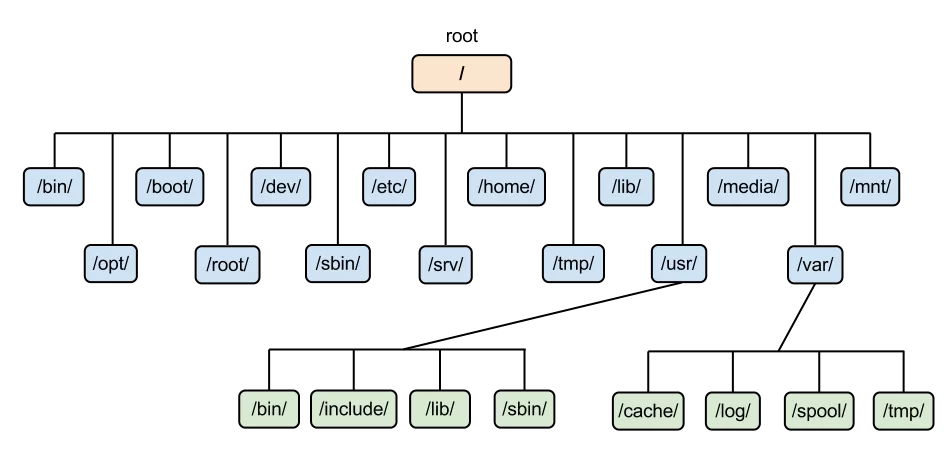
\includegraphics[width=\textwidth]{img/ch1/hfs.png}
%	\caption{Иерархия файловой системы}
%	\label{fig:galaxy}
%\end{figure}

%\keys{Сtrl + Shift + F}

%man -K IPX

%\texttt{man}

%\keys{Сtrl + Shift + F}

	
	\appendix
%	\include{appendixA}
	
	
%	\bibliographystyle{plain}
%	\bibliography{links}
	
\end{document}